\pagebreak

%-------------------------------------------------------------------------
\section{Research Plan}\label{sec:plan}
%-------------------------------------------------------------------------
\textcolor{red}{TODO: Jane: outline the approach taken by the team.}

%-------------------------------------------------------------------------
\subsection{Specific Aim 1: Develop frameworks for autonomous cognitive assistance in healthcare robots}\label{sec:plan-task1}
%-------------------------------------------------------------------------

\subsubsection{Automation of routine skills}
\textcolor{red}{TODO: Kris, Jacob}

This Task aims to develop an extensible foundation of hardware capabilities and reliable primitive skills that are applicable for the clinical domain.  We shall identify high-priority capabilities needed for a nursing robot.  Based on prior testing, we have already identified navigation, pick-and-place,
button-pressing, and surface cleaning as key tasks to be implemented.

Via  an  NSF  RAPID  Ebola  seed  grant,  the  Duke  team  developed  the  TRINA
platform (Figure 1) with the goal of enabling nurses and other workers to perform routine diagnostics and
care to infectious patients (i.e., Tuberculosis, Ebola, SARS, etc.) with zero personal exposure to pathogens. From a safe location, a human nurse can log on to TRINA to communicate with patients and other workers
via audio/video communication, navigate around obstacles, measure vital signs, bring food and medicine,
operate equipment, and move carts and furniture.

\paragraph{Primitive Skill Definition.} 
 By a primitive skill we refer to a finite-duration procedure that controls the low-level behavior of the robot in response to requested {\em skill parameters} and the {\em context} of the robot/environment state.  A skill has the following properties:
\begin{enumerate}
\item {\em A precondition} that dictates when it can potentially be applied.
\item {\em One or more postconditions} that may result, including correct operation (e.g., picking up requested item), incorrect operation (e.g., object cannot be picked up), or unexpected errors (e.g., object fell).
\item {\em Probability distribution over postconditions}.  These will be seeded with an unconditional distribution, and their conditional dependence on skill parameters and context will be learned over time through experience~\cite{Pasula_learningprobabilistic2004}.
\item {\em Real-time status information} may optionally be fed back to a human operator.
\item {\em Can be interruptable} or have skill parameters changed during execution.
\end{enumerate}  

Following~\cite{HauserTAMP2010}, the skill parameters may be either continuous or discrete variables.  Examples of continuous variables include target position for a navigation skill, a target object pose for a pick-and-place skill, or an area for a cleaning skill.  Discrete variables may include arm choice, object name, target location name, or button name.  Semantically specified discrete variables will index into a {\em knowledge base} that contains geometric models, physical information, and other properties of known objects, places, and robot poses.

\paragraph{2D Navigation.}  We use laser sensors and the Google Cartographer package to maintain 2D maps of the hospital floor. We have demonstrated collision-free omnidirectional navigation in the robot's local neighborhood.  We will extend this work to optimized  longer-term trajectories, as well as to named places.

\paragraph{Button pressing.} Buttons, knobs, and switches are ubiquitous in clinical environments.  In fact, nurses that we consulted during the development of TRINA 1.0 remarked that turning off alarms would be one of the most useful functions of the robot, since false alarms are frequent, irritating, and a waste of time, especially in quarantine environments in which PPE must be donned and doffed. Button pressing requires relatively precise maneuvering and force application, and hence teleoperation is relatively slow for this skill.

\begin{figure}
\centering
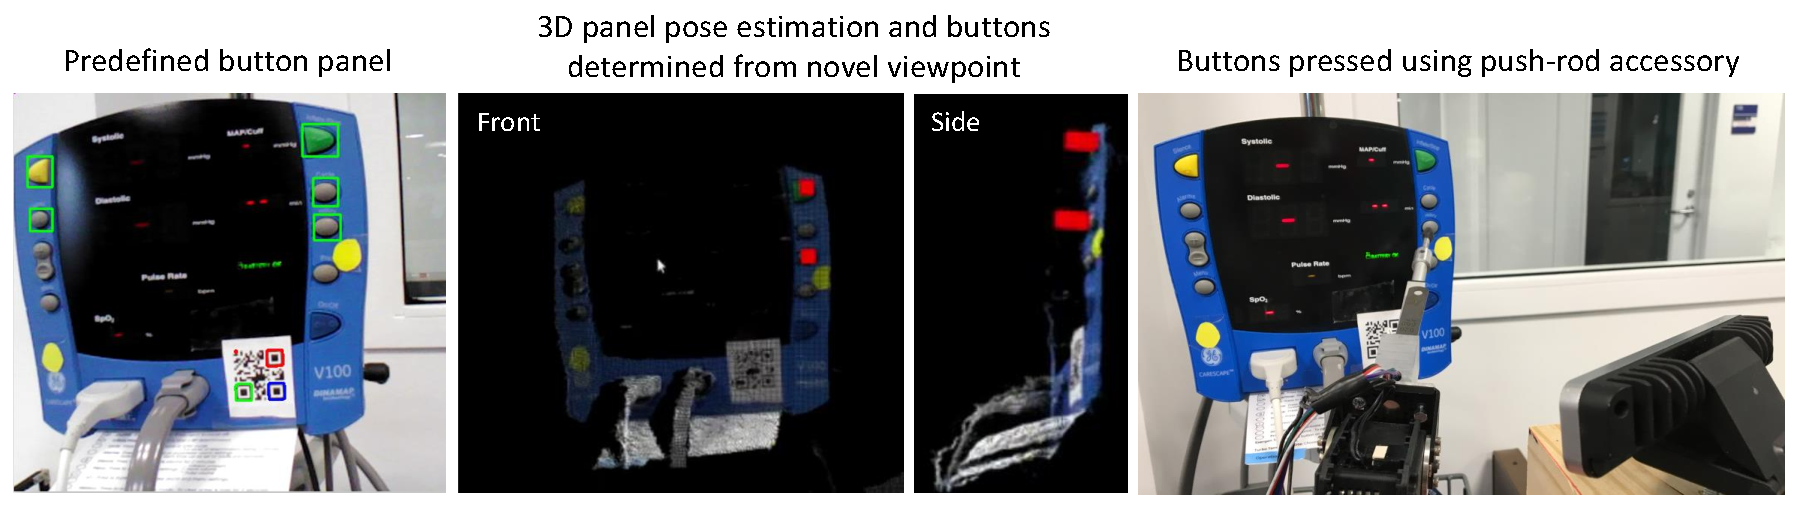
\includegraphics[width=0.9\textwidth]{fig/ButtonPressing.pdf}
\caption{Current work on a button pressing primitive skill. Left: A human prepares the environment by affixing a QR code, taking a single RGB+D image, and labeling button areas.  Middle and right: the system autonomously identifies button panels from novel viewpoints and presses the requested buttons using a precise pushing attachment.}
\label{fig:ButtonPressing}
\end{figure}

Current work is investigating strategies for autonomous button pressing.  We have already implemented a system for 3D mapping and identifying buttons in button panels (Figure~\ref{fig:ButtonPressing}) that requires a quick preparation of the clinical environment.  In the preparation phase, a 2\,cm$^2$ QR code is placed on the face of each button panel and a human gathers a clear picture and 3D scan of the button panel.  Then, the human labels the button panel and identifies and labels each button.  The segmented 3D scan, labels, and positions of each button are stored to a database.  This step takes approximately 1--3 minutes depending on the number of buttons on the panel, and can be performed with a laptop equipped with a 3D scanner or with the sensors on the robot.
%
For online detection, the robot is maneuvered close to the button panel, the QR code is detected by the robot's camera sensors and the robot moves into position to get a clear en-face view of the panel.  The 3D model of the panel is retrieved  from the database and registered to the RGB+D sensor data using the iterative closest points (ICP) algorithm.  Inverse kinematics is then used to press the button using the push-rod attachment of TRINA 1.0.  In preliminary tests, this method was able to operate 98.7\% of buttons and switches in a home and an office building~\cite{WangHauser2018}.
Once successfully integrated, button pressing will be decomposed into ``Localize Button'' and ``Operate Button'' primitive skills.

\paragraph{Pick-and-place.}  We will build on well-established techniques for autonomous grasping of objects on tabletops and placing them in collision-free locations, which will be useful for food tray preparation and waste disposal.   More advanced pick-and-place primitives may require identifying and separating objects in close contact (e.g., piles, stacks, against the edges of containers), transporting objects upright or with both hands, and manipulating deformable objects.

\paragraph{Surface cleaning.}  Discussions with nurses have also revealed that cleaning of bodily fluids is a frequently requested functionality of the robot.  We plan to enable the robot to clean a variety of surfaces like floors, tabletops, beds, medical equipment, and armrests via the primitive skills ``Prepare Cleaning Materials,'' ``Bulk Clean Area,'' ``Detail Clean Area,'' ``Dispose Cleaning Materials,'' and ``Clean Hands.'' Primitive areas will be defined as planar patches parameterized by location and shape, and cleaning will occur by moving the cleaning material along a fixed wiping pattern adapted to the size and location of the area.  More complex objects like beds and equipment will be defined as collections of multiple primitive areas.  If time permits, we will investigate vision algorithms for identifying soiled surfaces to clean more thoroughly.

\paragraph{Instrument placement against patient.} Instruments to collect vital signs should be placed against or near the patient in well-defined locations.  However, it takes a fair amount of training for human operators to determine where to position the robot's base and orient its appendages to reach those locations. The space near a bedridden patient is often cluttered, and for unresponsive or immobile patients the robot may need to also lift the patient's arm or move bed linens.  In this effort we plan to develop ``Navigate to Instrument Placement Location,'' ``Prepare Instrument Location,'' and ``Operate Instrument'' primitive skills.

\paragraph{Connect/disconnect tubing.} Nurses must frequently manipulate tubing for IVs, catheters, and suction containers to collect, replace, and dispose of fluids.  Attaching/detaching the connectors between tubes and containers (i.e., Luer-Lok) is a challenging task for teleoperation because it requires precise bimanual coordination of a combined twisting and pressing motion.  This primitive will use RGB-D sensing to identify the connector endpoints, connection status, and 3D reference coordinate system of each part.  Each part will be grasped by one of the end effectors, and then the appropriate twisting maneuver will be used.  To determine the necessary strength of twisting or pulling/pushing we will first attempt to use automated guarded moves with thresholds determined by connector type.  If this fails, we will fall back to a virtual fixture method~\cite{MOH2003} where the end effector paths are fixed, but progress along the path is guided by the human. 

\paragraph{Additional skill.} Once a basic suite of skills is generated, we will continue to consult with nurses to identify primitive skills that are necessary high-level clinical operation, high-priority, and/or repetitive.  Potential skills might include blood sample collection, opening sterile packaging, stripping bed linens, emptying waste containers, or pushing movable carts.  We will triage the development of recommended skills according to their clinical frequency and technical difficulty.

\paragraph{Capability testing.} Hardware upgrades to TRINA 2.0 will be evaluated using the same battery of clinical tasks in the nursing lab that were used to evaluate TRINA 1.0~\cite{LiTRINASystem2017}.  Trained nurse operators (n=12) will be asked to perform each task in direct teleoperation / shared control mode three times without direct line-of-sight (see Aim 3 for details on nurse recruitment). We will measure time and success rate. With the proposed upgrades, we hope to achieve at least 90\% of the identified nursing tasks (compared to 73\% in the prior version) and speed improvements of 30\% beyond the prior version.  Using the same protocol we will also evaluate novel tasks, such as wiping up a spill on the floor, which were physically impossible with TRINA 1.0 hardware.

Before inclusion in the library a primitive task will be evaluated for completeness of its specification and reliability levels.  Preconditions, postconditions, and error handling will be exhaustively unit-tested in the lab with a variety of objects and obstacle configurations, with at least 100 trials in total.  Our self-imposed quality requirements are that the preconditions, postconditions, and reported terminal status (success, failure, error) of the primitive to be correct at least 95\% of the time.



\subsubsection{Motion coordination assistance}
\textcolor{red}{TODO: Jane}

This task aims to study the motion-perception coordination developed through various teleoperation interfaces that differ in motion mapping. It also investigates the teleoperated motion coordination performed under passive, passive, active, and interactive perception. The teleoperated robot motion are decomposed to low-level motion primitives and abstract the high-level motion coordination plan, of which the features are used to measure and compare the motion-perception coordination developed through different teleoperation interface, and under various perception mode. We further study the regularity and variability of the developed motion coordination across teleoperation interfaces, to reveal the adaption of human motor control to robot motion and perception capabilities.

In this task, we focus on the behavior of expert teleoperators. We assume sufficient training, they have optimized the adaption of their motion-perception coordination strategies to the motion and perception capabilities of the teleoperated robots. Through this task, we aims to:

\begin{itemize}

\item Identify the sets and frequent combinations of teleoperated robot motion primitives developed through different teleoepration interface. 

\item Construct high-level representation of the teleoperated motion coordinations using symbols for abstract states and option. 

\item Develop novel performance metrics to quantitatively compare the motion primitives and task motion plan. 

\item Model the association of user's choice of camera views with the motion coordination plan to infer the motion-perception coordination strategy. 

\end{itemize}

\subsubsection{Adaptive task scheduling}
\textcolor{red}{TODO: Missy}

To address current challenges in scheduling and optimization of collaborative human-autonomy environments, we propose the development of the Collaborative Human-Autonomy Replanner for Medical Systems (CHARMS). Through models of the interdependencies between agents and impacts of agent failures, CHARMS will provide ``smart'' decision support for schedulers to identify and adapt to dynamic scheduling challenges in healtchare environments. Additionally, CHARMS will track ergonomic risk for human workers and failure risk for robots, enabling schedulers to manage both long and short term safety though proactive scheduling. 

CHARMS is a decision support tool that allows a supervisor to understand the impact of an agent (human or robot) ``failure'' across different work environments. CHARMS aids the supervisor in developing a contingency plan to mitigate production impact while maintaining a safe work environment. The development of CHARMS will utilize human-centered design, drawing upon interviews, demonstrations, and reviews with representative nursing personnel. CHARMS will be developed and tested in a mock hospital setting.

To date, there are no products available on the commercial product that can perform the full set of functions proposed for CHARMS. There are a variety of available industrial scheduling software packages that can assist with process sequencing and shift scheduling (e.g. Optessa, TACTIC, Lean Factory Management), but these are focused on human work scheduling and to our knowledge, none of these account for collaborative human-autonomy work architectures. 

Beyond considerations of ergonomic risk, from a dynamic rescheduling perspective unstructured collaborative environments provide greater flexibility in that both robots and humans can potentially act as a replacement for an absent human or malfunctioning robot. However, in these environments there are additional considerations for the certification of the agents in each of the tasks as well as the impacts of varying task completion efficiency on the productivity as a whole. To address related questions and provide a tool that incorporates a deep understanding of types of collaborative architectures and their resilience to perturbations in scheduling, the proposed work includes these primary elements:

\begin{enumerate}
    \item Determining a core set of design requirements and principles as well as detailed test and evaluation strategies in the development of a smart scheduling system for collaborative human-robot teaming in a manufacturing setting. This will include how a dynamic rescheduling system should be designed to capture the capabilities and limitations of both. We especially want to focus on the balance of work between robots and humans in order to minimize the ergonomic risk of human repetitive stress injuries.
    \item Creating an implementation of this smart scheduling systems with an emphasis on human-systems design principles and advanced optimization algorithms that focus on satisficing in the presence of uncertainty. In addition, these algorithms will be able to learn from the human coach to better tailor future solution recommendations.
    \item Conducting integrated testing utilizing actual robotic agents in a mock manufacturing environment.
    \item	Determining how the results from the design and tests in this representative environment can be extended to other healthcare settings. 
\end{enumerate}

The integration of robotic agents into CHARMS will focus on developing a set of representations of clinical workflow under collaborative human-autonomy environments. These representations will capture the temporal and physical interdependencies between tasks and workers (for both divisional and integrated collaborative human-autonomy environments). Additionally, CHARMS will be customizable to account for certifications, programming/re-programming restrictions, etc. that separate structured and unstructured environments and utilize these constraints in the generation of new replanning solutions.

Proposed functionalities based on initial discussions include:
\begin{itemize}
\item Characterization of a skill, rule, and knowledge-based cognitive reasoning taxonomy that will be needed to classify the basic requirements of collaborative tasks, both structured and unstructured (Rasmussen, 1983; Cummings M. , 2014).
\item Ability to request automated replanning and recommendations through optimization algorithms
\item Provide scheduling recommendations that account for the nature of the work environment (structured vs. unstructured), ergonomic risk, potential reliability issues, and that highlight potential safety compromises.
\item Ability for a supervisor to investigate changes to the schedule and coach the algorithms if needed
\item Provide alerts upon a change (both descriptive and predictive) in status of one of the robotic or human agents (e.g. malfunction or unexpected absence)
Our prior research on design of future systems and interfaces has included the development of the Hybrid Cognitive Task Analysis (hCTA) (Nehme, Scott, Cummings, \& Furusho, 2006). The hCTA methodology provides a principled approach to cognitive task and work analysis for systems that do not yet exist, such as the proposed integrated collaborative human-autonomy work environment. 
\end{itemize}

Specific goals for this task include: 
\begin{itemize}
    \item As a system designed to augment human decision-making capabilities, the design and implementation of CHARMS must consider the human as an integral part of the system and follow appropriate principles to maximize the human-machine performance. 
    \item The integration of collaborative human-autonomy environments as part of the CHARMS system must draw upon expertise in robotic systems, and these skills will be critical in the creation of a testbed for evaluating the system performance
    \item CHARMS will integrate with the onboard health and status monitoring of the robotic agents in order to provide the user with current information and alerts in case of a malfunction. These sources of information would be used as part of status visualizations for human decision makers in a decision support environment as well as inform the scheduling optimization algorithms. 
    \item The backbone of the CHARMS system focuses on replanning in uncertain environments, which will require careful consideration of approaches for schedule optimization or ``satisficing.''
    \item To provide a ``risk-aware'' scheduling system, CHARMS requires tracking and modeling of human ergonomic risk as well as robot reliability and prediction of necessary maintenance.
\end{itemize}

The evaluation of this task will utilize Duke Robotics facilities and personnel to test the implementation in a simulated tele-nursing environment with a robotic agent. This phase of lab testing will focus on the integration of the CHARMS system with the robotic and human agents and improve the understanding of scheduling in structured and unstructured environments. An initial version of the CHARMS software will be developed and installed on a computer system integrated with a set of robotic agents. This integration will include bi-directional communications allowing the central system to receive health and status information from the agents (such as a robotic malfunction) as well as distribute general tasking commands to the robotic agents. The development of this testing environment and the robotic worker actions will leverage prior work on validated human-robot interaction metrics (Cummings \& Donmez, 2013; Steinfeld, et al., 2006; Goodrich \& Schultz, 2007). Testing of the system will focus on a variety of conditions in the simulated environment to ensure proper functionality of the CHARMS system, including:
\begin{itemize}
    \item Identification of a malfunction of a robot worker
    \item Supervisor input of human worker absence or incapacity.
    \item Rescheduling of tasks and agents due to the unavailability of an agent, under several architectures:
    \begin{itemize}
        \item Divisional and structured: Tasks performed in series, only allow human replacements of human workers, requires specified maintenance distribution time to repair for robotic agents.
        \item Divisional and unstructured: Tasks performed in series, allow both human and robotic replacements for robotic workers, only human replacements for human workers
        \item Integrated and structured: Tasks performed simultaneously, only allow human replacements of human workers, requires specified maintenance distribution time to repair for robotic workers
        \item Integrated and unstructured: Tasks performed simultaneously, allow both human and robotic replacements for robotic workers, only human replacements for human workers
    \end{itemize}
\end{itemize}

%-------------------------------------------------------------------------
\subsection{Specific Aim 2: Model the socioeconomic impact of healthcare robots}\label{sec:plan-task2}
%-------------------------------------------------------------------------
\subsubsection{Economic and labor market analysis}
\textcolor{red}{TODO: Alex}

\subsubsection{Attitudes of personnel to robotics}
\textcolor{red}{TODO: Missy, Jeanine, or Ryan?}

\subsubsection{Bias and disparate impact analysis}
\textcolor{red}{TODO: Jeanine}

%-------------------------------------------------------------------------
\subsection{Aim 3: Model the interaction between autonomy and impact}\label{sec:plan-task3}
%-------------------------------------------------------------------------

\subsubsection{Design of the human-autonomy interface}
\textcolor{red}{TODO: Missy}

\subsubsection{Effects of interface and autonomy on bias}
\textcolor{red}{TODO: Jeanine}

\subsubsection{Formulate best practices}
\textcolor{red}{TODO: Jane}



\subsection{Milestones and Timeline}

